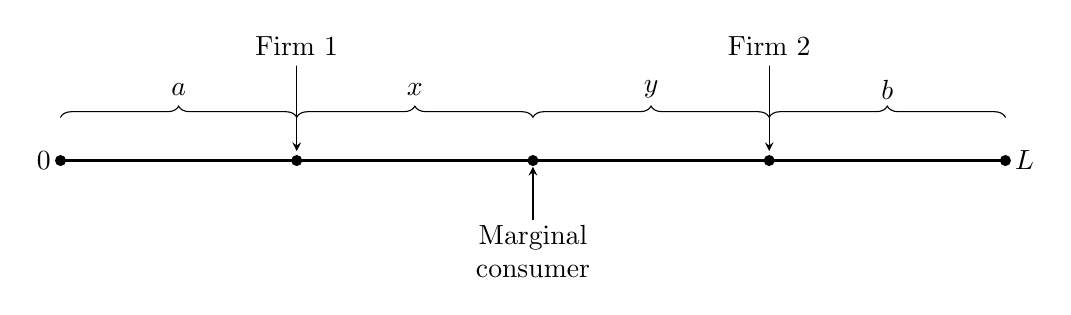
\begin{tikzpicture}[>=stealth, line cap=round]

    % --- Key x-positions (edit these to change spacing) ---
    \def\xO{0}
    \def\xFone{3}
    \def\xMC{6}
    \def\xFtwo{9}
    \def\xL{12}

    % --- Baseline ---
    \draw[thick] (\xO,0) -- (\xL,0);

    % --- Points ---
    \fill (\xO,0) circle (2pt);
    \fill (\xFone,0) circle (2pt);
    \fill (\xMC,0) circle (2pt);
    \fill (\xFtwo,0) circle (2pt);
    \fill (\xL,0) circle (2pt);

    % --- End labels ---
    \node[left]  at (\xO,0) {$0$};
    \node[right] at (\xL,0) {$L$};

    % --- Braces above segments: a, x, y, b ---
    \draw[decorate, decoration={brace, amplitude=4pt}]
    (\xO,0.55) -- (\xFone,0.55) node[midway, yshift=10pt] {$a$};

    \draw[decorate, decoration={brace, amplitude=4pt}]
    (\xFone,0.55) -- (\xMC,0.55) node[midway, yshift=10pt] {$x$};

    \draw[decorate, decoration={brace, amplitude=4pt}]
    (\xMC,0.55) -- (\xFtwo,0.55) node[midway, yshift=10pt] {$y$};

    \draw[decorate, decoration={brace, amplitude=4pt}]
    (\xFtwo,0.55) -- (\xL,0.55) node[midway, yshift=10pt] {$b$};

    % --- Firm labels with downward arrows ---
    \node at (\xFone,1.45) {Firm 1};
    \draw[->] (\xFone,1.20) -- (\xFone,0.12);

    \node at (\xFtwo,1.45) {Firm 2};
    \draw[->] (\xFtwo,1.20) -- (\xFtwo,0.12);

    % --- Marginal consumer label with upward arrow from text to point ---
    \node[align=center] at (\xMC,-1.15) {Marginal\\consumer};
    \draw[->] (\xMC,-0.75) -- (\xMC,-0.08);

\end{tikzpicture}